  \section{RC lux}

  \subsection{The beginning}

  \begin{frame}
          \frametitle{The beginning}
  \begin{itemize}[<+->]
  \item \textbf{Where? } Cosmology and subatomic physics laboratory in Grenoble
  \item \textbf{Who? } Pascal Sortais, plasma and ion sources specialist
	\begin{quotation}
	 I was, then, convinced that I could improve UV lamps technology. It was enough to adapt particle accelerators technologies to lower energies\footnote{Le journal la CNRS, \url{http://www2.cnrs.fr/presse/journal/2853.htm}}.
	\end{quotation} 
  \item \textbf{When? } 25 January 2006, RC Lux is created
	\end{itemize}
  \end{frame}

  \subsection{The steriliser}

  \begin{frame}
          \frametitle{The steriliser}
  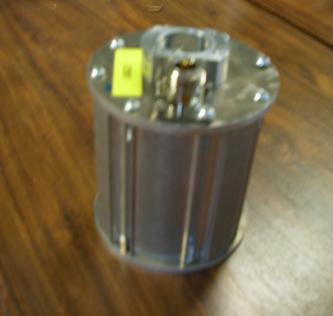
\includegraphics[height=4.5cm, width=4cm]{images/steriliser.jpg}
\hspace{0.5cm}
\begin{minipage}{0.5\linewidth}
 Award winner of most innovative technologies for environment
\end{minipage}
  

  \end{frame}
